\section{Layerwise Spatial Dynamics}
\label{app:layer-dynamics}

We use the all-layer hidden-state distances saved during the Qwen 7B
experiments to examine how spatial sensitivity changes across depth. This
analysis does not intervene directly on internal activations and should
therefore be interpreted as layerwise sensitivity rather than activation
patching.

Localization improves sharply in the later half of the model. Average patch
AP on grounded examples rises from $0.365$ at hidden-state index 15 to $0.781$
at index 21, while top-one target hit rises from $32.5\%$ to $92.5\%$.
Top-three target hit reaches $97.5\%$. From index 21 onward, $80.0\%$ of
examples keep the same highest-ranked patch through every remaining hidden
state, and average adjacent-layer top-patch stability is $95.9\%$.

\begin{figure}[t]
\centering
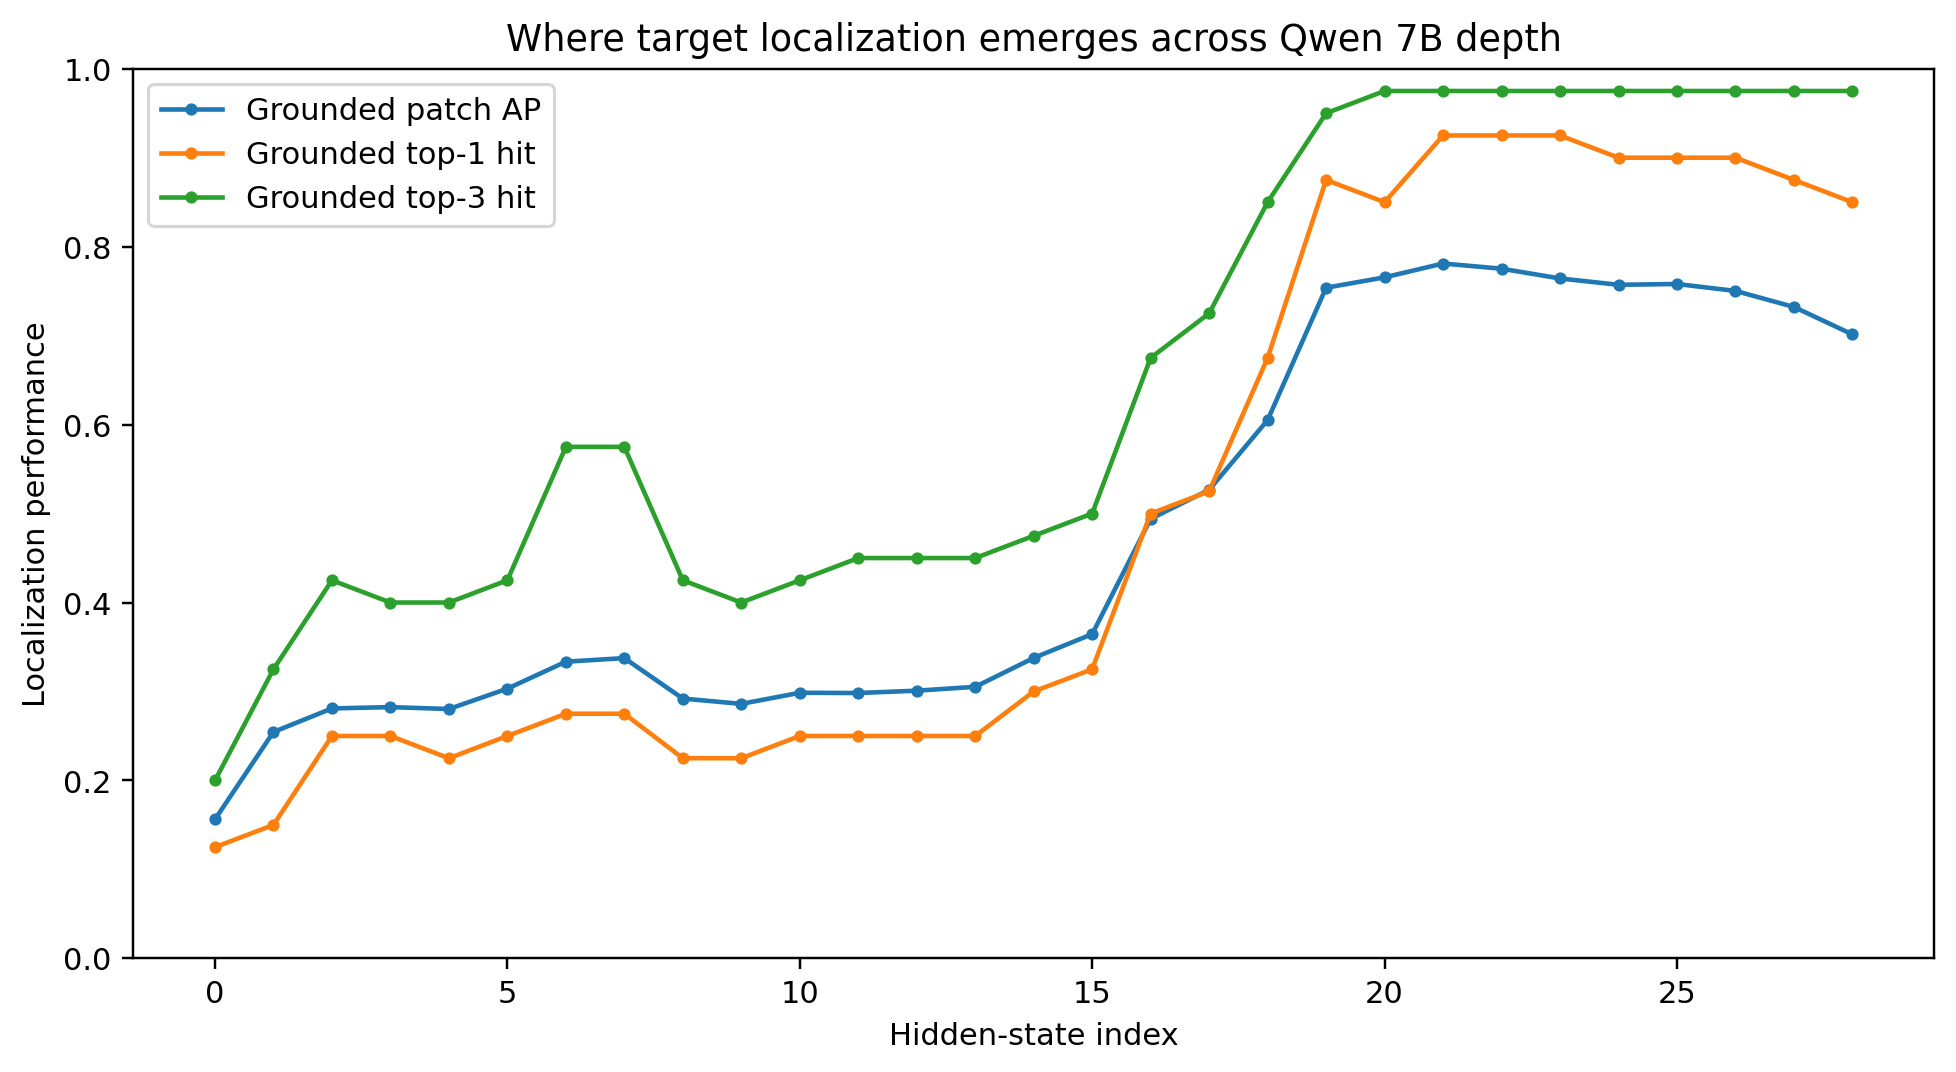
\includegraphics[width=\linewidth]{figures/localization_across_depth.png}
\caption{Target localization across Qwen 7B hidden-state depth. Target-aligned
patch rankings emerge sharply in later hidden states and remain strong through
the final representation.}
\label{fig:localization-depth}
\end{figure}

The airport service-vehicle example gives a concrete view of this transition.
Earlier hidden states alternate among several regions. At hidden-state index
15, the strongest patch switches to the ground-service vehicle and remains
there through the final state. Its share of the total positive sensitivity
increases from $6.5\%$ at index 15 to $38.0\%$ at index 24.

\begin{figure}[t]
\centering
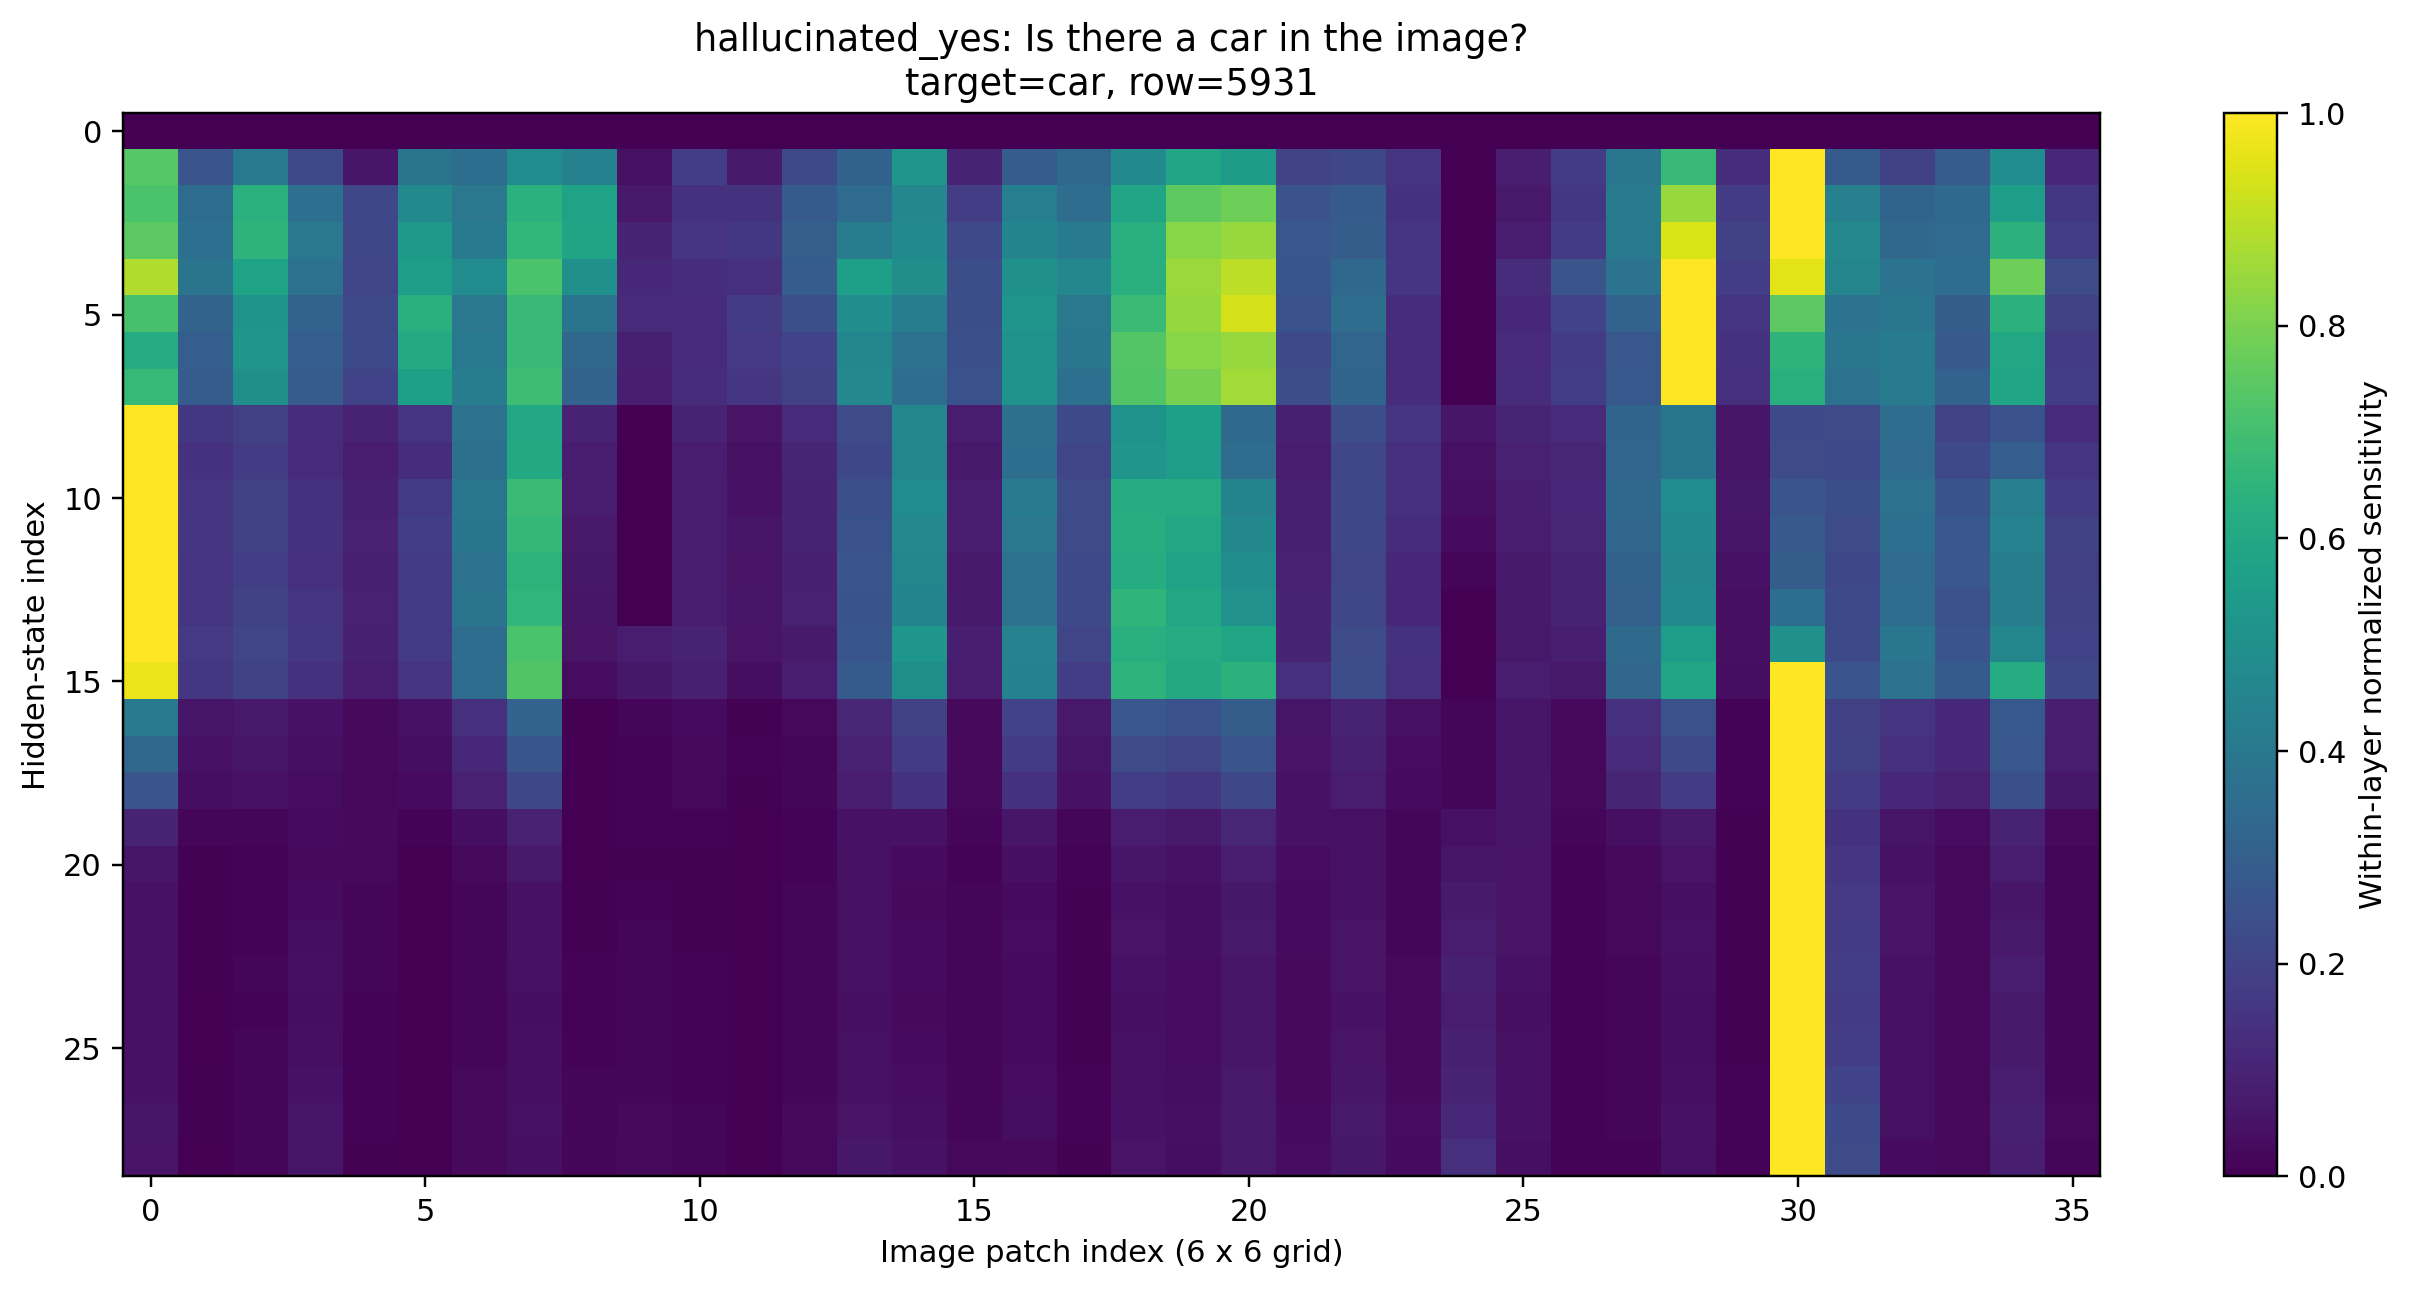
\includegraphics[width=\linewidth]{figures/layer_by_patch_airport.png}
\caption{Layer-by-patch sensitivity for the airport hallucination. Each row is
normalized within a hidden-state index. The service-vehicle patch becomes
dominant in the later half of the model and remains stable thereafter.}
\label{fig:airport-layer-patch}
\end{figure}

These results support the main framework by showing that the later
answer-position representations used for patch ranking contain a stable,
target-aligned spatial signal. They do not establish the exact hidden state at
which the model causally reads a region; that stronger claim would require
activation patching.
